\documentclass[11pt]{article}
\usepackage{graphicx} % Required for inserting images

\usepackage[utf8]{inputenc}

\usepackage{amsmath,amsthm, amssymb}
\usepackage[margin=3cm]{geometry}
\usepackage{mathtools}
\usepackage{dsfont}
\usepackage{xcolor}
\usepackage{algorithm,algpseudocode}
\usepackage{todonotes}
\usepackage{nicefrac}
\usepackage{mathrsfs}
\usepackage{tikz}

\usepackage{subcaption}

\usepackage{hyperref}



\usepackage{thm-restate}

\usepackage{etoc}

\usepackage{setspace}
% \setstretch{1.125}


%%%%%%%%    THEOREM DEFINITIONS AND RESTATABLE
% \newcounter{claim}
% \setcounter{claim}{0}
\newtheorem{theorem}{Theorem}
\newtheorem{lemma}[theorem]{Lemma}
\newtheorem{corollary}[theorem]{Corollary}
\newtheorem{claim}{Claim}
\newtheorem{dependency}{Dependency}
\newtheorem{definition}[theorem]{Definition}

\newcommand{\matt}[1]{\todo[color=red!50, prepend, caption={Matt}, tickmarkheight=0.25cm]{#1}}
% \newcommand{\matt}[1]{\textcolor{red}{{\Large TODO:} #1}}

\newcommand{\on}{\rm on}
\newcommand{\off}{\rm off}
\newcommand{\haar}{\text{Haar}}

%%%%%%%%    NOTATION DEFINITIONS FOR EASIER WRITING
\newcommand{\ket}[1]{|#1\rangle}
\newcommand{\bra}[1]{\langle #1|}
\newcommand{\braket}[2]{\langle #1|#2\rangle}
\newcommand{\ketbra}[2]{| #1\rangle\! \langle #2|}
\newcommand{\parens}[1]{\left( #1 \right)}
\newcommand{\brackets}[1]{\left[ #1 \right]}
\newcommand{\abs}[1]{\left| #1 \right|}
\newcommand{\norm}[1]{\left|\left| #1 \right|\right|}
\newcommand{\diamondnorm}[1]{\left| \left| #1 \right| \right|_\diamond}
\newcommand{\anglebrackets}[1]{\left< #1 \right>}
\newcommand{\overlap}[2]{\anglebrackets{#1 , #2 }}
\newcommand{\set}[1]{\left\{ #1 \right\}}
\newcommand{\ceil}[1]{\left\lceil #1 \right\rceil}
%\newcommand{\openone}{\mathds{1}}
\newcommand{\expect}[1]{\mathbb{E}\brackets{#1}}
\newcommand{\EE}{\mathbb{E}}
\newcommand{\TT}{\mathcal{T}}

\newcommand{\variance}[1]{\textit{Var} \brackets{ #1 }}
\newcommand{\prob}[1]{{\rm Prob}\left[ #1 \right]}
\newcommand{\bigo}[1]{O\left(#1\right)}
\newcommand{\bigotilde}[1]{\widetilde{O} \left( #1 \right)}
\newcommand{\ts}{\textsuperscript}
\newcommand{\deltaM}{\Delta_{\text{M}}}

\DeclareMathOperator{\Tr}{Tr}
\newcommand{\trace}[1]{\Tr \brackets{ #1 }}
\newcommand{\partrace}[2]{\Tr_{#1} \brackets{ #2 }}
\newcommand{\complex}{\mathbb{C}}

%%%%% COMMONLY USED OBJECTS
\newcommand{\hilb}{\mathcal{H}}
\newcommand{\partfun}{\mathcal{Z}}
\newcommand{\identity}{\mathds{1}}
\newcommand{\gue}{\rm GUE}
\DeclareMathOperator{\sinc}{sinc}
\DeclareMathOperator{\hermMathOp}{Herm}
\DeclareMathOperator{\im}{Im}
\DeclareMathOperator{\diag}{diag}
\newcommand{\herm}[1]{\hermMathOp\parens{#1}}

\usepackage{authblk}

\begin{document}

\title{The Thermodynamic Cost of Ignorance:\\ Thermal State Preparation with One Ancilla Qubit}

\author[1]{Matthew Hagan}
\affil[1]{University of Toronto, Department of Physics, Toronto ON, Canada}
\author[2,3,4]{Nathan Wiebe}
\affil[2]{University of Toronto, Department of Computer Science, Toronto ON, Canada}
\affil[3]{Pacific Northwest National Laboratory, Richland WA, USA}
\affil[4]{Canadian Institute for Advanced Research, Toronto ON, Canada}
\date{\textbf{Extended Abstract}}
\maketitle
Thermal states are fundamental primitives for many quantum algorithms, ranging from quantum chemistry and materials simulations to Semi-Definite Program (SDP) solvers. They are also of utmost importance in physics, as systems tend to generically equilibrate to the temperature of their surrounding environments. Understanding the problem of thermalization, or how systems approach thermal states, is therefore a critical task for both the physics of open quantum systems and quantum computer science. In our paper we propose a quantum algorithm that is capable of preparing thermal states for arbitrary systems at arbitrary temperatures and compiles to simple Hamiltonian evolution circuits, thereby providing both new methods for thermal state preparation on quantum computers and an extension of the open quantum systems model of Repeated Interactions to arbitrary systems. We are not only able to show correctness of the algorithm, meaning that the output is $\bigotilde{\epsilon}$ close in trace distance to the thermal state, but also are able to bound the runtime needed to reach this output in two scenarios: the first in which a user has perfect knowledge of the eigenvalue differences $\lambda_S(i) - \lambda_S(j)$ and the other in which these differences are completely unknown and the user is forced to sample uniformly at random from some interval containing all the differences.

Our algorithm is inspired by the classical Hamiltonian Monte Carlo (HMC) algorithm, which is a modification of the original Metropolis-Hastings algorithm that eliminates random walk behavior. HMC works by extending the state space of the system of interest to include momentum variables and then utilizes time-evolution of the extended Hamiltonian to transition to new states. As the probability of accepting new samples scales like the exponential of the energy difference, and since Hamiltonian evolution naturally preserves energy, every sample is theoretically accepted ignoring numerical integration errors. By implementing a quantum version of HMC, which does not have a rejection filter, we are able to avoid the dealbreakers of Marriot-Watrous rewinding \cite{temme2011} or other weak measurement schemes \cite{jiang2024quantummetropolissamplingweak} present when trying to adapt standard Metropolis-Hastings algorithms to quantum computers.

The quantum algorithm we developed can be summarized as follows. First, prepare the system in a state diagonal in the Hamiltonian basis, the maximally mixed state or a Haar random pure state are sufficient, and a single ancilla qubit in a thermal state $\frac{e^{-\beta H_E}}{1 + e^{-\beta \gamma}}$, with an energy gap $\gamma$ that can be chosen uniformly at random from the interval $[0, 4\norm{H_S}]$. Then, choose an interaction term with Haar random eigenvectors and I.I.D Gaussian eigenvalues and add it to the system and environment Hamiltonians with a coupling constant $\alpha$. Finally, simulate the system-environment Hamiltonian wth interaction for a time $t$ and then trace out the ancilla qubit. This yields our overall channel
\begin{equation}
    \Phi(\rho) = \mathbb{E}_G \partrace{\rm env}{e^{-i(H_S + H_E + \alpha G) t} \left( \rho \otimes \frac{e^{-\beta H_E}}{\partfun_E(\beta)} \right) e^{+i(H_S + H_E + \alpha G) t} },
\end{equation}
which is then repeated $L$ times. The main goal of our analysis is to show that there exist choices of $\alpha$, $t$, and $L$ that lead to an $\bigotilde{\epsilon}$ approximation of the thermal state.

One of the main appeals of our algorithm is it's simplicity. The above construction relies solely on time-independent simulation of the original system Hamiltonian, and to simulate the random interaction it is sufficient to utilize Haar 2-designs and random Pauli-$Z$ rotations. Further, the construction is optimal with respect to the number of ancilla qubits used. This is in stark contrast to many existing 

One of the main advantages of our algorithm is the simplicity, the only ingredients necessary to compile this channel to an implementable quantum circuit is time-independent Hamiltonian simulation, Haar 2-designs, and random Pauli-$Z$ rotations. The clearest point of comparison with existing algorithms would be recently developed Linbladian based methods \cite{chen2023quantumthermalstatepreparation, gilyen2024quantumgeneralizationsglaubermetropolis}. These techniques involve constructing a Linbladian based around coherent sums of Fourier weighted jump operators, which are nontrivial to implement circuits for. 

To show that this channel prepares the thermal state we use a weak-coupling expansion that is second order in the coupling constant $\alpha$ to compute the transition elements $T_{j, i} =  \frac{\alpha^2}{2} \frac{\partial^2}{\partial \alpha^2}\bra{j} \Phi\ketbra{i}{i}) \ket{j}$. Computing these bounds is the most technical contribution in our paper, but boils down to repeated applications of Duhamel's formula along with second moment Haar integrations. We then show that the total mapping up to second order can be represented exactly as a Markov chain over the system eigenbasis. This representation as a Markov chain allows us to then provide arguments about the fixed points and convergence time of the channel $\Phi$ and is dependent on the tuning of the ancilla gap $\gamma$.

Before we discuss our algorithm and the results we obtain, we would like to outline other approaches to preparing thermal states, also known as Gibbs sampling. Recent developments in the field \cite{chen2023quantumthermalstatepreparation, gilyen2024quantumgeneralizationsglaubermetropolis, motlagh2024ground, motta2019, ding2024single} can be categorized into a handful of approaches. Many of the most general techniques \cite{chen2023quantumthermalstatepreparation, gilyen2024quantumgeneralizationsglaubermetropolis}, general with respect to the range of systems capable of being prepared and the temperature range they can be cooled to, are based on simulating models of open quantum systems, namely Davies generators of a Linbladian superoperator \cite{davies1974markovian}. These algorithms have seen a marked improvement in recent years, ranging from ground state preparation routines with single-ancilla overhead \cite{ding2024single} to the first constructions that satisfy a discrete-time detailed balance condition \cite{gilyen2024quantumgeneralizationsglaubermetropolis}. Most previous algorithms are not based on physical models of open quantum systems, such as \cite{zhang2023dissipative} which utilizes weak measurements or \cite{poulin2009sampling, jiang2024quantummetropolissamplingweak} which rely on Quantum Phase Estimation.
  
One of the main drawbacks to the Linbladian based approaches is the sheer complexity of the resulting algorithms. These algorithms tend to rely on coherently weighted sums of Heisenberg evolved jump operators and the construction of circuits to simulate the resulting Linbladians is nontrivial, as mentioned in Section 1.2 of \cite{gilyen2024quantumgeneralizationsglaubermetropolis}. Further, these algorithms tend to require logarithmically more ancilla qubits to allow for the addition of jump operators whereas our routine explicitly utilizes only a single ancilla qubit. Turning to ground states specifically, there exists single ancilla algorithms \cite{ding2024single}  but we remark that our channel is the first general purpose thermal state preparation routine for finite $\beta$ that utilizes only one qubit explicitly. 

The most closely related thermal state preparation algorithm is that by Shtanko and Movassagh \cite{shtanko2023preparingthermalstatesnoiseless}. They propose two algorithms, one tailored to a specific class of Hamiltonians and another more general algorithm. The first couples the system to a large bath of ancilla qubits via random $k$-local Pauli terms but is only proven to work for input Hamiltonians satisfying the Eigenstate Thermalization Hypothesis (ETH). The second couples the system to a bath of ancilla qubits via random circuit rotations. This second algorithm works for more generic Hamiltonians, but has a prohibitively high failure probability and involves an extra rejection step similar, but not identical to, Temme et al \cite{temme2011}. Further, both of these algorithms have runtimes with explicit $\beta$ scaling which leads to a breakdown of their analysis in the $\beta \to \infty$ limit. Improving the analysis of these algorithms to more general Hamiltonians and to the ground state limit are important open problems, as mentioned in the conclusion of \cite{shtanko2023preparingthermalstatesnoiseless}. Our algorithm resolves both of these open problems, working for not only arbitrary non-degenerate Hamiltonians but with explicit runtime bounds in the ground state, $\beta \to \infty$, limit. 

% Given the ubiquity of thermal state preparation, also known as Gibbs sampling, there exists a plethora of algorithms 


% algorithms for the problem on classical computers have seen active development since the origins of the Metropolis-Hastings algorithm in the 1950's. Algorithms for preparing thermal states on quantum computers are much less developed and are stymied by a lack of physical understanding of how generic systems approach thermal equilibrium. Recently there has been rapid development of quantum algorithms for thermal state preparation based on two different physical theories, one by simulating Linbladian evolution of the Davies Linbladian and the other by simulating the time evolution of Eigenstate Thermalization Hypothesis (ETH) satisfying Hamiltonians. The rest of this section will provide an overview of existing algorithms for thermal state preparation. 

% The first algorithms proposed for preparing thermal states on quantum computers rely on phase estimation to directly work in the Hamiltonians eigenbasis or attempt to mimic the Metropolis-Hastings algorithm. Some drawbacks to the phase estimation approach is that phase estimation requires a doubling of the number of qubits and has no clear path to analyzing special case Hamiltonians beyond the exponential time required for the worst-case scenario. Previous Metropolis-Hastings algorithms have struggled to handle the sample filtering required in the classical algorithm and not only require complicated techniques such as Marriot-Watrous rewinding but also have questionable proofs of correctness.

% Recently developed physically inspired methods offer much improved algorithms over existing techniques. Chronologically, the first algorithm developed by Shtanko and Movassagh utilizes time evolution of the system while coupled to a thermal bath. These techniques offer conceptually simpler circuits than either of the existing approaches mentioned, as they essentially only require Hamiltonian simulation routines. Two drawbacks to this approach are as follows. The first is that one algorithm they propose only works for ETH satisfying Hamiltonians and explicitly scales with $\beta$, meaning that the exact ground state limit is unattainable. The second algorithm proposed does work for generic Hamiltonians, but the convergence method used is a relative entropy bound that has a prohibitively high failure probability for low precision $\epsilon$ of the output state.

% More recently, a variety of algorithms \cite{chen2023quantumthermalstatepreparation, gilyen2024quantumgeneralizationsglaubermetropolis} based on Linbladian approaches have been show to prepare thermal states for generic systems. These approaches are based on a physical model for thermalization known as a Davies generator. These algorithms are generic, satisfy the Kubo-Martin-Schwinger (KMS) conditions for thermal state fixed points (in some settings exactly, in others approximately), and can be shown to be efficient for ETH satisfying Hamiltonians. Some drawbacks of these algorithms is that they are fairly complex and involve procedures such as coherently weighted Fourier transforms of the input Hamiltonian and operator square roots, meaning that compiling these routines to specific circuits is very nontrivial. A further complication is that the runtime of many of these algorithms explicitly depend on a mixing time, which is difficult to compute for arbitrary systems.

\section{Main Results}
We provide both extensive numeric and rigorous theoretic analysis of our proposed algorithm. Analytically we study our channel for four scenarios, two specific and two applied. The specific systems we study are single qubit systems and truncated harmonic oscillators. For the single qubit system we are able to obtain an explicit bound on the total simulation time required to reach a trace distance of $\bigotilde{\epsilon}$ to the thermal state. For the harmonic oscillator we are able to show that the thermal state is the unique fixed point, provided knowledge of the oscillator gap $\Delta$, and are able to bound the total simulation time required as $\bigotilde{\frac{\dim_S^9}{\Delta \epsilon^{2.5} \lambda_\star(\beta) }}$, where $\lambda_\star(\beta)$ is the spectral gap of the Markov transition matrix. We are further able to show that in the ground state limit this gap can be computed as $\lim_{\beta \to \infty} \lambda_\star(\beta) = 1$. 

Our other two analytic results hold for arbitrary non-degenerate Hamiltonians and the requirement on non-degeneracy is relatively mild and can be lifted fairly easily but complicates our proof techniques unnecessarily. For these Hamiltonians we prove convergence of the channel in two scenarios: one in which no knowledge of the eigenvalue differences beyond an upper bound on the spectral norm is present and the other in which the eigenalue differences are known exactly. We restate these theorems below in a more informal setting than present in the technical manuscript.
\begin{theorem}[Zero Knowledge Thermal State Prep - Informal] \label{thm:zero_knowledge}
    Let $H_S$ be a non-degenerate Hamiltonian of dimension ${\rm dim}_S$, $\rho$ any input state such that $[\rho, H_S] = 0$, $\gamma$ chosen uniformly from $[0, 4 \norm{H_S}]$, and
    let $\rho_{\rm fix}$ denote the unique fixed point of the Markovian dynamics underlying $\Phi$. The following statements hold.
    \begin{enumerate}
\item For finite $\beta$ the thermal state is a controllably approximate fixed point
    \begin{equation}
        \norm{\rho_S(\beta) - \EE_\gamma \Phi_\gamma(\rho_S(\beta))}_1 \in \bigo{\alpha^2 t e^{\beta \min_{i \neq j} \set{\lambda_S(i) - \lambda_S(j)}}}.
    \end{equation}
    \item   The parameter settings for any $\beta\in [0,\infty]$ and error tolerance $\epsilon \in (0,2]$
    \begin{align}
        \alpha = \frac{\delta_{\min}^4 \epsilon^{3} \widetilde{\lambda}_\star(\beta)^{3}}{\dim_S^7 \norm{H_S}^3}, ~t = \frac{\dim_S^2 \norm{H_S}}{\epsilon \widetilde{\lambda}_\star(\beta) \delta_{\min}^2}, \text{ and } L \in \bigotilde{\frac{\dim_S^{14} \norm{H_S}^6}{\epsilon^5 \delta_{\min}^6 \widetilde{\lambda}_\star(\beta)^{6} }},
    \end{align}
    where $\widetilde{\lambda}_\star(\beta)$ is the spectral gap of the underlying Markov chain, are sufficient to guarantee $\norm{\rho_{\rm fix} - \left(\EE_\gamma \Phi_\gamma \right)^{\circ L}(\rho)}_1 \in \bigotilde{\epsilon}$.
   \item    In the $\beta \to \infty$ limit the fixed point is exactly the ground state and the spectral gap is lower bounded by a constant
    \begin{equation}
        \lim_{\beta \to \infty} \rho_{\rm fix} = \ketbra{1}{1} \text{ and } \lim_{\beta \to \infty} \widetilde{\lambda}_\star(\beta) = 2 \int_{0}^{-\delta_{\min}t/2} \sinc^2(u) du \ge 2.43.
        \end{equation}

    \end{enumerate}
\end{theorem}
The second Theorem we prove in the paper is a refinement of the above result in the scenario where eigenvalue differences are known exactly.
% \begin{theorem}[Perfect Knowledge Thermal State Prep] \label{thm:perfect_knowledge}
%     Assume the same setup in the Zero Knowledge Theorem but now let $\gamma$ be a random variable with distribution $\prob{\gamma = \Delta(i,j)} = \frac{\eta_\Delta(i,j)}{\binom{\dim_S}{2}}$ where $\eta_\Delta(i,j)$ is the number of times a particular eigenvalue difference appears. For any $\beta\in [0,\infty]$ the thermal state can be prepared with controllable error
%     \begin{equation}
%         \norm{\rho_S(\beta) - \left(\EE_\gamma \Phi_\gamma \right)^{\circ L}(\rho)}_1 \in \bigotilde{\epsilon}
%     \end{equation}
%      with the following parameter settings
%      \begin{align}
%          \alpha &= \frac{\delta_{\min} \epsilon^{1.5} \widetilde{\lambda}_\star(\beta)^{1.5}}{\dim_S^7}, t = \frac{\dim_S^2}{\delta_{\min} \epsilon^{0.5} \widetilde{\lambda}_\star(\beta)^{0.5}},\text{ and } L \in \bigotilde{\frac{\dim_S^{14}}{\epsilon^2 \widetilde{\lambda}_\star(\beta)^3}},
%      \end{align}
%      where $\widetilde{\lambda}_\star(\beta)$ is the spectral gap of the rescaled transition matrix $\EE_\gamma T_\gamma  \cdot \frac{\binom{\dim_S}{2}}{\widetilde{\alpha}^2}$. 
%      This gives the total simulation time required as
%      \begin{equation}
%          L \cdot t \in \bigotilde{\frac{\dim_S^{16}}{\delta_{\min} \epsilon^{2.5} \widetilde{\lambda}_\star(\beta)^{3.5}}}.
%      \end{equation}
%      All of the above conditions hold in the ground state limit as $\beta \to \infty$ and further we can compute a lower bound on the spectral gap of the rescaled transition matrix as
%      \begin{equation}
%          \lim_{\beta \to \infty} \widetilde{\lambda}_\star(\beta) = \min_{i > 1} \sum_{j < i} \eta_\Delta(i,j) \ge 1.
%      \end{equation}
% \end{theorem}
\begin{theorem}[Perfect Knowledge Thermal State Prep - Informal] 
    Assume the same setup as the Zero Knowledge Thermal State Prep Theorem but now let $\gamma$ be a random variable sampled from the distribution $\prob{\gamma = \Delta(i,j)} = \frac{\eta_\Delta(i,j)}{\binom{\dim_S}{2}}$, where $\eta_\Delta(i,j)$ is the number of times a particular eigenvalue difference appears. In this scenario the fixed point is exactly the thermal state $\rho_{\rm fix} = \rho_S(\beta)$ for all $\beta$ and the time $t$ and number of interactions $L$ can be reduced to 
    \begin{align}
         t = \frac{\dim_S^2}{\delta_{\min} \epsilon^{0.5} \widetilde{\lambda}_\star(\beta)^{0.5}}\text{ and } L \in \bigotilde{\frac{\dim_S^{14}}{\epsilon^2 \widetilde{\lambda}_\star(\beta)^3}},
     \end{align}
     giving an asymptotic reduction in the total simulation cost of $\widetilde{O}\left({\frac{\|{H_S}\|^7}{\delta_{\rm min}^7 \epsilon^{3.5}
\lambda_\star(\beta)^{3.5}}}\right)$. 
\end{theorem}

One of the key features of our algorithm is the simplicity of the resulting channel which is easy to implement on a quantum computer and easy to study numerically on classical computers. Although we have more extensive investigations of the channel for the single qubit and harmonic oscillator in the paper, below we include two plots: one that demonstrates the error performance of the channel and another that investigates the dependence of the runtime on the knowledge of the eigenvalues. For the error performance the main takeaway is that by going beyond the weak-coupling regime we can achieve much faster cooling, indicating that our analysis has plenty of room for improvement. One possible extension could be to utilize the fast convergence of strong coupling and then reducing the coupling constant to ``fine-tune" the output to a lower error. Turning to the second plot, we study the impacts of noise added to our Perfect Knowledge theorem. We fix specific values of $\alpha, \epsilon, t,$ and $\beta$ and then measure the minimum number of interactions needed to prepare the thermal state. We then vary the amount of Gaussian noise added to the eigenvalue samples for $\gamma$ from the exact distribution and plot how this affects the minimum number of interactions needed. We extend the standard deviation of the noise all the way to the spectral radius of the Hamiltonian, which is then essentially a uniformly generated sample. The takeaway from this plot is that at very noisy samples for $\gamma$ we are still able to prepare the thermal state for even realistic systems, we use a chain of 3 hydrogen atoms as our Hamiltonian of interest, as predicted by our Zero Knowledge theorem. The decrease in simulation time shows that heuristic values for the eigenvalues can significantly reduce the simulation cost, in this scenario by almost half. 

\begin{figure}
    % \begin{subfigure}
    % \end{subfigure}
    \begin{subfigure}{0.49\linewidth}
        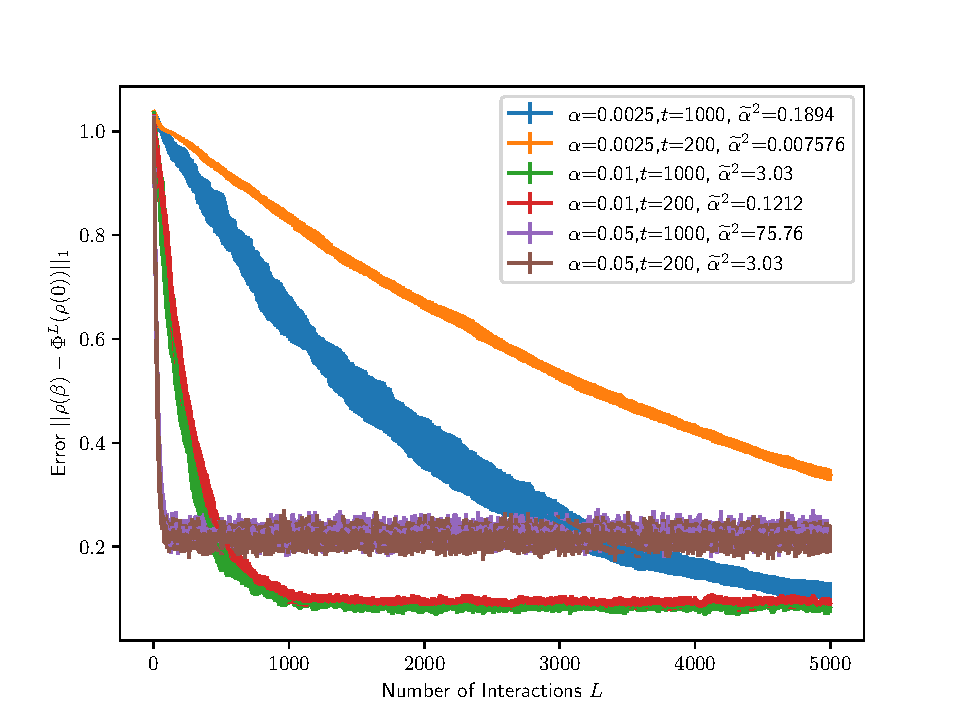
\includegraphics[width=\textwidth]{numerics/data/error_vs_interaction_h2_chain_1.pdf}
        \caption{Hydrogen-2 Chain Error}
    \end{subfigure}
    \begin{subfigure}{0.49\linewidth}
    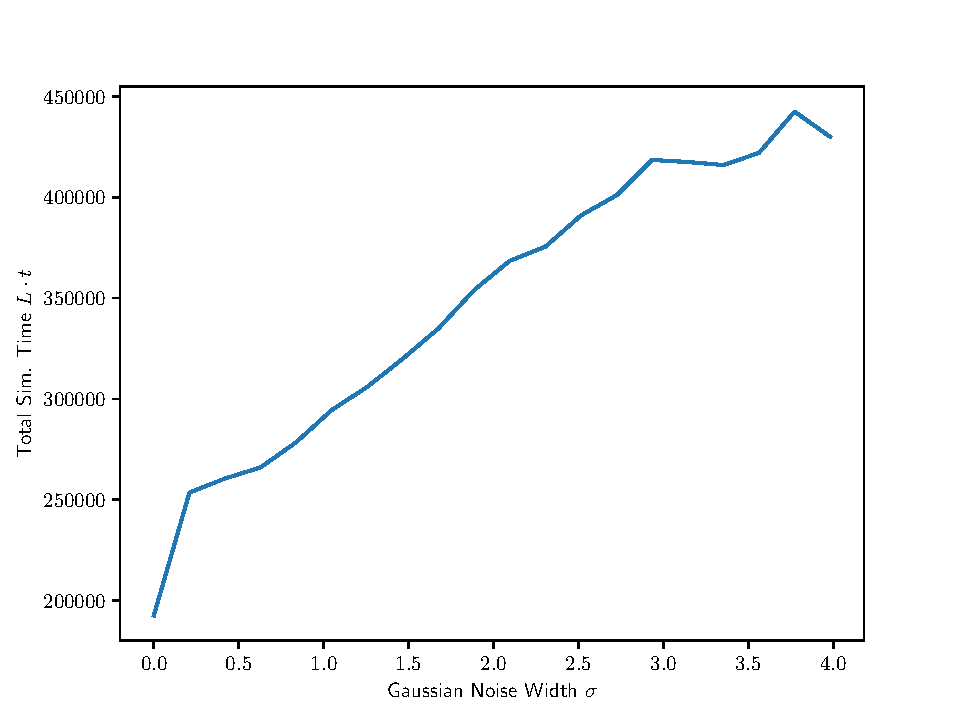
\includegraphics[width=\textwidth]{numerics/h3_chain_with_noise_3.pdf}
    \caption{Hydrogen-3 Chain Simulation Time}
    \end{subfigure}
\end{figure}

% Thermal states are fundamental primitives for many quantum algorithms, ranging from quantum chemistry to SemiDefinite Program (SDP) solvers. As they approach the ground state as the temperature of the thermal state approaches 0, they are very computationally difficult to prepare but also incredible resources for probing various properties, such as entanglement structure, of the Hamiltonian under study. How quantum systems efficiently approach thermal equilibrium is a major open question from both a physics perspective, as in how do realistic quantum systems interact with an environment to cool to the same temperature as the environment, and a computational perspective, meaning how can we prepare thermal states for a given Hamiltonian on a digital, fault-tolerant quantum computer. 

% From the physics perspective there exist a few proposed methods for how generic systems may approach thermal equilibrium. The Eigenstate Thermalization Hypothesis (ETH) is a leading mechanism for understanding how many-body systems that do not interact with an external environment can appear thermal for any single particle. This model however is not typically accommodating for environment interactions and it is still an open problem to classify all Hamiltonians that satisfy the assumptions needed, hence the "Hypothesis" in the name. Linbladian dynamics are used to describe environments that are typically much larger than the system. This framework works well in the weak system-enivornment coupling regime and with "Markovian" environments, which can be thought of as large environments that are not effected by the interaction with the system. As a result these models tend to break down in strong coupling and small environment regimes. The Repeated Interactions (RI) framework was developed describe very small environments that are repeatedly refreshed. This method is relatively difficult to study for arbitrary systems and as a result most results have been for small systems, such as single qubits or three-level systems. 

% From the computational perspective there are algorithms that work for generic Hamiltonians, such as phase estimation based approaches or Metropolis-Hastings inspired approaches. In the past few years there has been rapid development of physics based approaches, some that work for ETH satisfying Hamiltonians and others that are based on Linbladian simulations and work for all systems. In our paper we develop a new thermalization procedure that relies solely on Hamiltonian simulation of the unprocessed Hamiltonian of interest.   

\bibliographystyle{unsrt}
\bibliography{bib}
\end{document}